\section{Introduction}
In the past decade, with the introduction of technology that can store huge amounts of data, a large amount of musical data is increasingly available to public on different application platforms such as Spotify. As the number of musical data in our phones and Internet keeps increasing, there is a need to characterize each music track so that finding a specific song in a large archive of music would not be a problem. Musical genres are commonly used to describe and characterize songs for music information retrieval. Pachet suggests that genre of music can be the best general information for music content description \cite{Pachet:2003}. Hence, a system that can classify musical genres can solve the problem of locating a specific sound track on any device. 

The only problem with musical genre classification is the fact that the definition of genre is very subjective by its nature and there exists thousands of genres or sub-genres. It is also important to note that, the definition of music genre tends to change with time, as what we call Rock song today is very different from the rock songs twenty years ago. Even though musical genres are subjective, there are certain features that can easily distinguish between different genres. By using features such as distribution of frequency or the number of beats, it is possible to classify main genres of music. For classification of musical genres, various approaches have been proposed. Unfortunately, most of these approaches have been proven to show accuracy around 60-70\%. Therefore, new approaches that can maximize classification accuracy must be considered.  

Hence, we try to improve the classification accuracy of music genre classification of audio signals in this work. Specifically, we use a wide range of machine learning algorithms, including k-Nearest Neighbor (k-NN) \cite{KNN:2009}, k-Means Clustering \cite{Clustering:2001}, Support Vector Machines \cite{SVM:2006}, Gaussian Mixture Models \cite{Pachet:2003} and different types of Neural Networks to classify the following 5 genres: metal, classical, blues, pop, country. 

Our main goal in this study is to maximize the classification accuracy of 5 genres and compare different methods of machine learning for classification of audio signals. We use state-of-the-art machine learning platforms such as PyTorch \cite{PyTorch:2017} to introduce deep learning into our project. We experiment with different neural network architectures and types of neural network. Moreover, we use Mel Frequency Cepstral Coefficients (MFCC) \cite{MFCC:2011} to extract useful information from musical data as recommended by past work in this field.
To summarize, we make three main contributions in this paper:
\begin{itemize}
  \item We experiment with a wide range of machine learning algorithms and state their classification accuracy for 5 different genres. 
  \item We propose a method for feature extraction and audio processing that is dependent on both MFCC and PCA. We also discuss the significance of such methods. 
  \item We report experimental data that describe the overall effectiveness of our classification methods by including confusion matrices. 
\end{itemize}

Our experimental results suggest that Convolutional Neural Networks produced the best classification results, with 90\%, whereas k-Nearest Neighbor algorithm outputted the least accurate classification, with 81\%. We observed that Support Vector Machines and Gaussian Mixture Models are also quite effective, with accuracy results around 85\%. Additionally, the super classifier we created by combining GMM, SVM, k-NN, and a simple 3-layer neural network showed promising results . Furthermore, we found that 16 dimensions is the best reduction of our data through Principal Component Analysis. 

\section{Related Work}\label{sec:related}

The development of music genre classification has been increasing rapidly in the past decade. Many approaches have been proposed that build different models for genre classification. Some approaches concentrate on the processing of audio signals, whereas some approaches try to combine audio signals with lyrics from each musical track to increase accuracy. Some of the related work to our project is presented below. 

Firstly, Tzanetakis and Cook \cite{GTZAN:2002} introduced different feautres to organize musical tracks into a genre by using k-NN and Gaussian Mixture Model (GMM) methods. Three different feature sets for speaking to tumbrel surface, rythmic substance and pitch substance of music signse were suggested. They also introduced a dataset for music genre classification (GTZAN Dataset \cite{GTZAN:2002}), which is widely used today in many project, including ours. 

Furthermore, Aucouturier and Pachet \cite{Pachet:2003} used GMM and utilized Monte Carlo procedures for evaluation of KL divergence, which was used in a k-NN classifier. They conveyed some significant component sets for musical information retrieval that we use in our work, specifically the MFCC. 

Apart from models such as GMM or k-NN, Feng \cite{Feng:2016} proposed an approach that uses Restricted Boltzmann machine algorithm to build deep belief neural networks. By generating more dataset from the original limited music tracks, he shows great improvement in the classification accuracy and describes the significance of neural networks for music genre classification. 

Xing et. al. \cite{Xing:2016} proposes a similar approach that uses convolutional neural networks. By combining max and average pooling to provide more more statistical information to higher neaural networks and applying residual connections, Xing et. al. \cite{Xing:2016} improves the classification accuracy on the GTZAN data set greatly. Li, Chan and Chun \cite{Chun:2010} recommend a very similar technique to concentrate musical example included in audio signals by using convolutional neural networks. They present their revelation of the perfect parameter set and best work on CNN for music genre classification.

Finally, Smaragdis and Whitman \cite{Smaragdis:2002} presents a very interesting musical style identification scheme based on simultaneous classification of auditory and textual data. They combine musical and cultural features of audio tracks for intelligent style detection. They suggest that addition of cultural attributes in feature space improves the proper classification of acoustically dissimilar music within the same style.

As compared to these works, we do a comparative study of genre classification where we experiment with 7 different classifiers. Even though our feature extraction method is very similar to other works, not many works use PCA right after extracting MFCC features. Furthermore, to the best of our knowledge, this project is the first to create a super classifier, which is basically an ensemble method that uses 4 different classifiers and combines their predictions. Finally, in terms of classification accuracy, our experimental results are better than previous works that also used only 4 or 5 genres instead of 10. Specifically, there are only a few works that were able to be beat the 90\% accuracy threshold. Hence, we believe our controbution to music genre clasification research is significant.  
%%%%%%%%%%%%%%%%%%%%%%%%%%%%

\section{Proposed Approach}\label{sec:approach}
% Dataset --> Feature Extraction --> Dimensionality Reduction --> Algorithms 
\subsection{Musical Dataset}
For musical data, Marsyas is an open source software framework for Music Information Retrieval with the GTZAN Genre Collection Database, which has 10 genres and each genre has 100 30-second audio tracks. All the tracks are 22050 Hz Mono 16-bit audio files in .au format. 

For this project, we chose five distinct genres; classical, metal, blues, pop, country. Hence, our dataset was 500 songs total, from which we used 80\% for training and 20\% for testing. We chose five very distinct genres as previous works \cite{Chun:2010} suggest more than 5 genres can decrease accuracy a lot and introduces many problems. 

\subsection{Feature Extraction: Mel Frequency Cepstral Coefficients (MFCC)}
Previous works \cite{MFCC:2011} on music classification and processing of audio signals directed us to use MFCC (Mel Frequency Cepstral Coefficients) as a method for feature extraction so that time domain waveforms can be represented in the frequency domain in a mel-scale. For the process of MFCC, we first computed the spectogram of each waveform by using Fast Fourier Transform and a Hamming Window. Then, we mapped each frequency to mel scale, as mel scale is the best scale for human ears. The mel spectogram of a song from each genre is shown on Figures 1 through 5, so that the difference between each genre can be visualized. After computing the mel-spectograms of each song, we applied discrete cosine transform (DCT) and then removed the very high frequency values from our data. At the end, we had an MFCC array of each song, where we stacked all them together, created appropriate labels for each genre and constructed our training and testing datasets. As stated, we used 80\% for training and 20\% for testing our classifiers. 

% Figure 1-5 --> Mel-spectograms 

\begin{figure}
\begin{center}
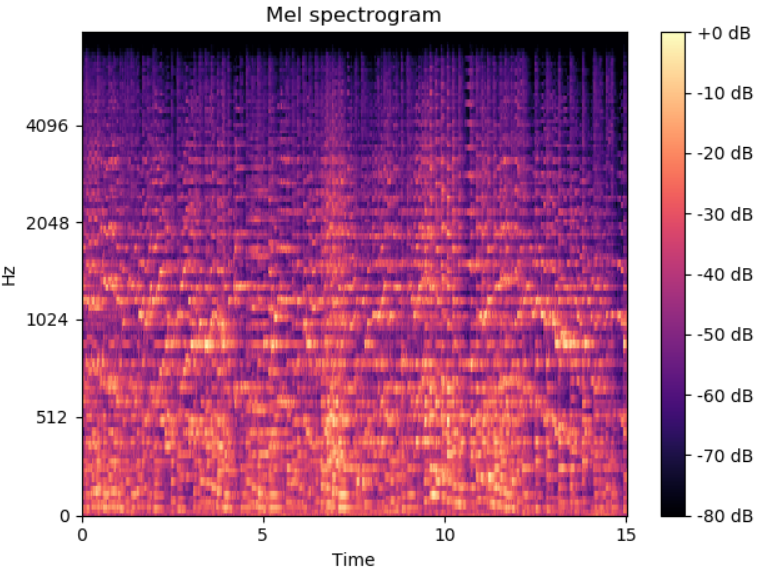
\includegraphics[scale=0.2]{./figures/classical.png}
\end{center}
\caption
{
Mel-spectogram of classical genre.
}
\label{fig:big_picture1}
\end{figure}

\begin{figure}
\begin{center}
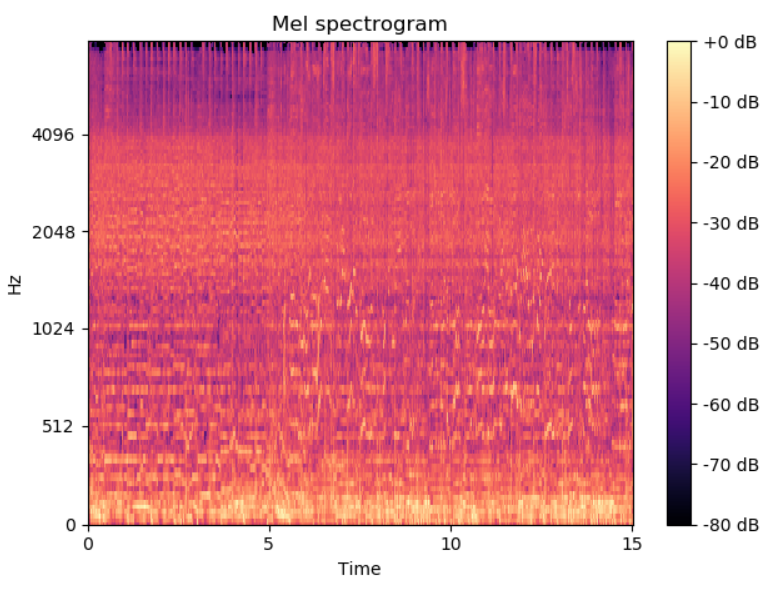
\includegraphics[scale=0.2]{./figures/metal.png}
\end{center}
\caption
{
Mel-spectogram of metal genre.
}
\label{fig:big_picture2}
\end{figure}

\begin{figure}
\begin{center}
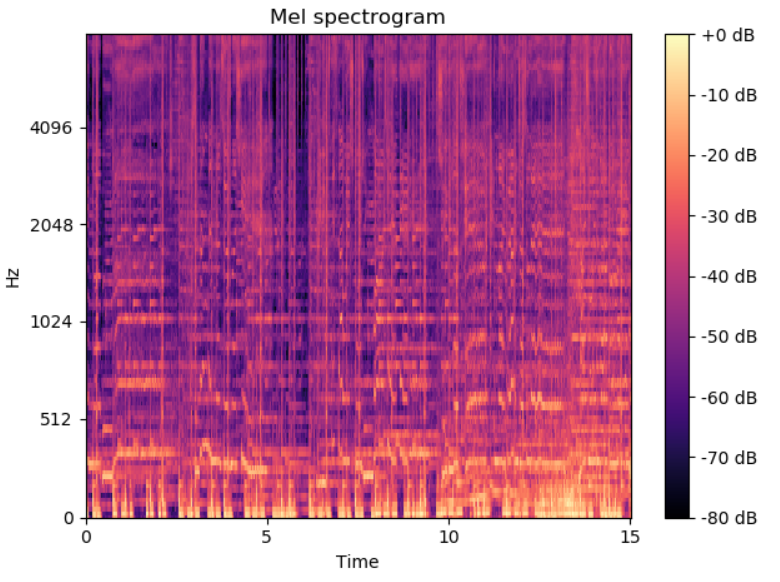
\includegraphics[scale=0.2]{./figures/pop.png}
\end{center}
\caption
{
Mel-spectogram of pop genre. 
}
\label{fig:big_picture3}
\end{figure}

\begin{figure}
\begin{center}
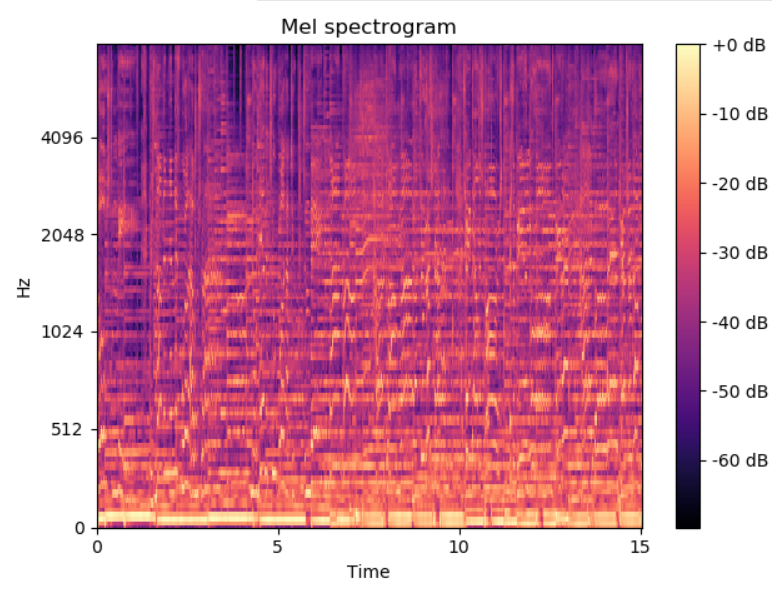
\includegraphics[scale=0.2]{./figures/country.png}
\end{center}
\caption
{
Mel-spectogram of country genre. 
}
\label{fig:big_picture4}
\end{figure}

\begin{figure}
\begin{center}
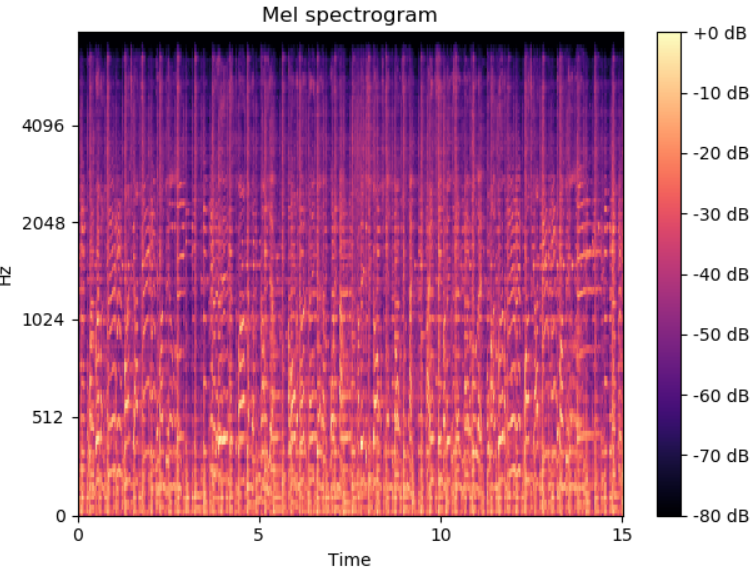
\includegraphics[scale=0.2]{./figures/blues.png}
\end{center}
\caption
{
Mel-spectogram of blues genre. 
}
\label{fig:big_picture5}
\end{figure}

\subsection{Dimensionality Reduction with Principal Component Analysis (PCA)}
After feature extraction and construction of final dataset, we thought of using dimensionality reduction before putting out data through classifiers. Since Principal Component Analysis (PCA) is a well-known and effective method for reduction of dimensions, we used PCA on our dataset. A realistic choice for number of reduced dimensions is to visualize the data with different PCA values and then pick the minimum dimension that can keep at least 95\% of the significant components. The visualization of our data with respect to different PCA dimensions and the corresponding eigenvectors is shown on Figure 6. Note that figures 7 and 8 also present a visualization of each genre in 2 and 3 dimensions. After extensive analysis of the visualization, and experimenting with out classifiers, we reduced the dimensionality to 16. Even though 16 dimensions performed very well on classifiers such as k-NN or SVM, we had to use much bigger dimensions for our neural network, since neural networks need much more data in practice. 

% Figure 6 --> PCA vs. Eigenvecs
\begin{figure}
\begin{center}
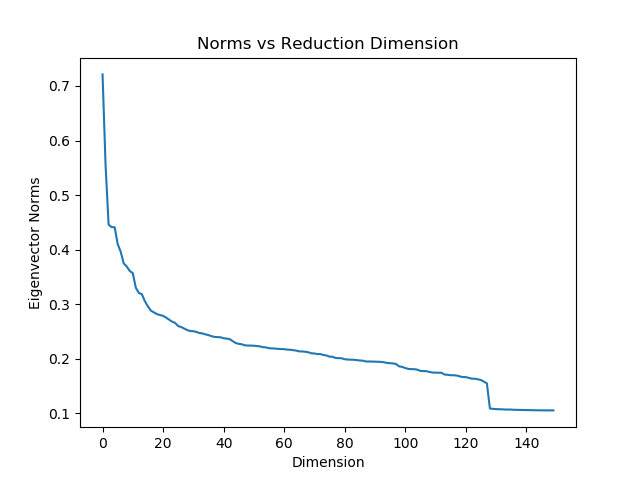
\includegraphics[scale=0.3]{./figures/pca_eig.png}
\end{center}
\caption
{
Norms of eigenvectors of our data plotted with respect to PCA dimensions. Note that we only want to keep the most significant components.
}
\label{fig:big_picture5}
\end{figure}

% Figure 7 --> 2-dimensional plt 
\begin{figure}
\begin{center}
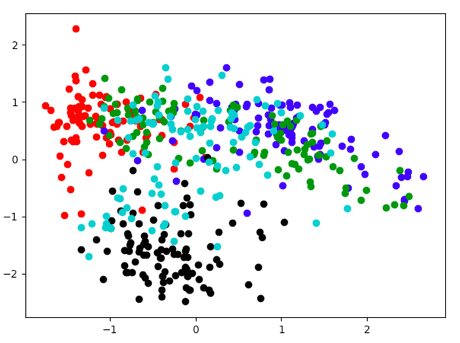
\includegraphics[scale=0.3]{./figures/2_d_plot.png}
\end{center}
\caption
{
2-dimensional scatter plot of our data with different genres. 
}
\label{fig:big_picture5}
\end{figure}
% Figure 8 --> 3-dimensional plt 

\begin{figure}
\begin{center}
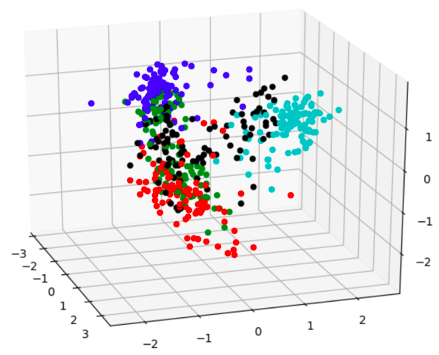
\includegraphics[scale=0.3]{./figures/3_d_plot.png}
\end{center}
\caption
{
3-dimensional scatter plot of our data with different genres. 
}
\label{fig:big_picture5}
\end{figure}

\subsection{Machine Learning Algorithms}
\subsubsection{\textbf{K-Nearest Neighbor (K-NN)}}
The first algorithm we used is the very famous and effective k-closest neighbors algorithm. k-NN is a non-linear algorithm that can detect direct or indirect spread of data. It is very effective for huge amounts of data. One downside of k-NN is the fact that it makes hard decisions and might produce low classification accuracy. Other than that, k-NN is computationally expensive since it does not learn any data, and it has to compute the distance for every point in prediction. We used Euclidean distance for k-NN, which produced good results. After our experiments, we also found that k=5 produced the best results. 

\subsubsection{\textbf{Support Vector Machines (SVM)}}
The second technique we used is the support vector machine (SVM), which is a directed organization method that discovers the extreme boundary splitting two classes of information \cite{SVM:2006}. The idea behind the algorithm is to project data onto a higher dimensional space in order to separate classes in a better way. We used Radial Basis Function (RBF) for our kernel for SVM and change the penalty to three. 

\subsubsection{\textbf{K-Means Clustering}}
We attempted to use clustering by Kmeans which produces a hard assignment to a cluster for each data point. We initialized this algorithm randomly and assigned each point to the nearest cluster by using euclidean distance, and updated each cluster mean. This algorithm proceeds iteratively until the cluster means do not change. We found that reducing the data to 16 dimensions produced the best results. One challenge we had was evaluating clustering methods. We found that we could use Fowlkes-Mallows score to give an accuracy.

\subsubsection{\textbf{Gaussian Mixture Models (GMM)}}
After KMeans clustering, we attempted to improve the clustering accuracy by implementing Gaussian Mixture Models. Each gaussian cluster has a mean and associated covariance, and each data point has a probability associated with each cluster. This gives soft assignments, which are usually better to deal with. We used sklearn's GMM class and experimented with different initialization techniques and covariance. 

\subsubsection{\textbf{Simple 3-layer Neural Network}}
After implementing different wll-known classifiers, we wanted to experiment with neural networks since they generally produce promising results in machine learning applications. Firstly, we used PyTorch to process our dataset and constructed a 3-layer neural network that uses ReLU for nonlinearity. Then, we experimented with different PCA dimensions and different hidden layer sizes to produce the best accuracy. The architecture of the network that gives the best classification results is shown in Figure 9. 

%%--> Figure 9.3-layer NN Architecture

\subsubsection{\textbf{Convolutional Neural Network (CNN)}}
We also wanted to experiment with Convolutional Neural Networks, since they can be much more effective than a simple 3-layer neural network or any other classifier. The downside of CNN is the fact that it requires a great deal of hyperparameter tuning. We experimented with different PCA dimensions, convolution kernel sizes, nonlinearity functions and the amount of dropout that we have to add. After testing our classifier with many different parameters, we were able to get a very good accuracy for music genre classification. The architecture that produced the best accuracy is shown on Figure 10. 
%%--> Figure 10. CNN Architecture

\subsubsection{\textbf{Super-Classifier (SC)}}
After completing a few other methods, we decided to try an ensemble method where we took 4 classifiers (GMM, k-NN, SVM, 3-layer Neural Network) and for each data point in the testing set, ran each classifier and took the most common label as the prediction. This produced better results than each of the methods individually. The motivation behind this implementation of the super classifier was the fact that each individual classifier had different least and most accurate genres. 

\section{Experimental Results}\label{sec:results}
\subsection{Experiment Setup}
The experimental setup for computation of classification accuracies were quite simple. After extracting features of our data through MFCC and applying PCA, we saved our training and testing datasets into a file, so that we do not have to do all the computations again. Then, we wrote a script that loads the training and testing datasets, and then puts the training data as an input to each of our classifiers with the corresponding genre labels. After training on each classifier, we computed predictions of each song and compared each label with its ground truth. Finally, we outputted the classification accuracy of each classifier and their confusion matrices, which are shown in Figure 11 through 18.

\subsection{Classification Accuracy}

\begin{table}
\begin{center}
\caption{Classification results of each classifier} 
\begin{tabular}{ p{1.9cm} p{1.1cm} p{2.8cm} p{2.8cm}}
 \emph{Classifier Type} & \emph{Accuracy}  & \emph{Most Accurate Genre} & \emph{Least Accurate Genre}\\
 \hline
 K-NN & 81\% & Metal & Classical \\
 SVM & 84\% & Classical & Country \\
 K-Means & 83\% & Classical & Country \\
 GMM & 85\% & Metal & Blues \\
 3-layer NN & 88\% & Classical & Pop \\
 CNN & 90\% & Classical & Blues \\
 SC & 88\% & Classical  & Country  \\
\end{tabular}
\end{center}
\end{table}

\begin{figure}
\begin{center}
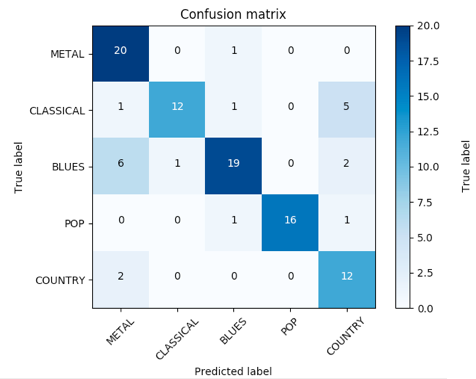
\includegraphics[scale=0.3]{./figures/confusion_knn.png}
\end{center}
\caption
{
Confusion matrix for k-Nearest Neighbors.
}
\label{fig:big_picture5}
\end{figure}

\begin{figure}
\begin{center}
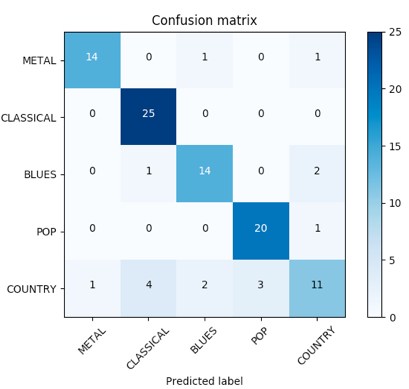
\includegraphics[scale=0.3]{./figures/confusion_svm.png}
\end{center}
\caption
{
Confusion matrix for Support Vector Machines.
}
\label{fig:big_picture5}
\end{figure}

\begin{figure}
\begin{center}
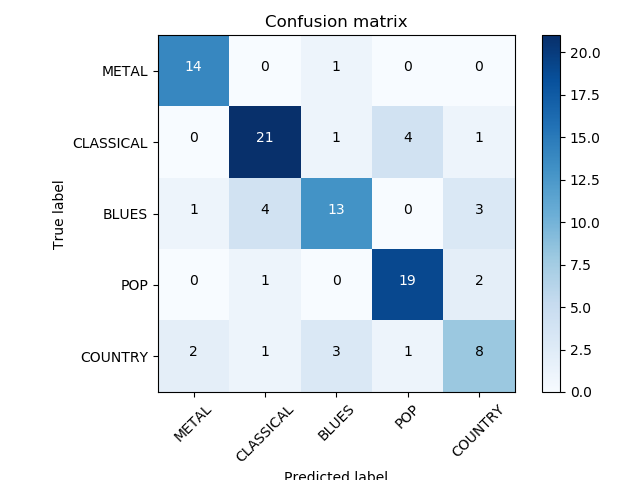
\includegraphics[scale=0.25]{./figures/confusion_kmeans.png}
\end{center}
\caption
{
Confusion matrix for K-Means Clustering. 
}
\label{fig:big_picture5}
\end{figure}

\begin{figure}
\begin{center}
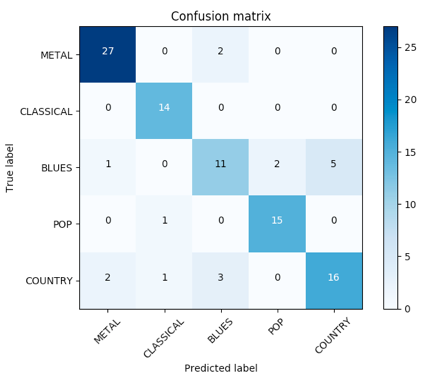
\includegraphics[scale=0.3]{./figures/confusion_gmm.png}
\end{center}
\caption
{
Confusion matrix for Gaussian Mixture Models. 
}
\label{fig:big_picture5}
\end{figure}

\begin{figure}
\begin{center}
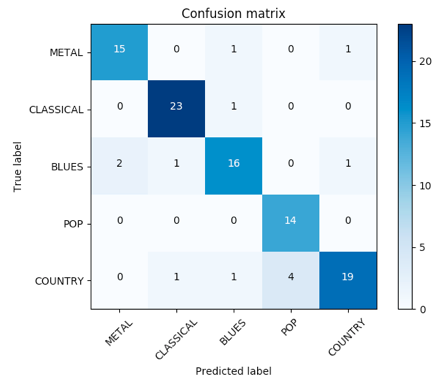
\includegraphics[scale=0.3]{./figures/confusion_simple_NN.png}
\end{center}
\caption
{
Confusion matrix for 3-layer Neural Network.
}
\label{fig:big_picture5}
\end{figure}

\begin{figure}
\begin{center}
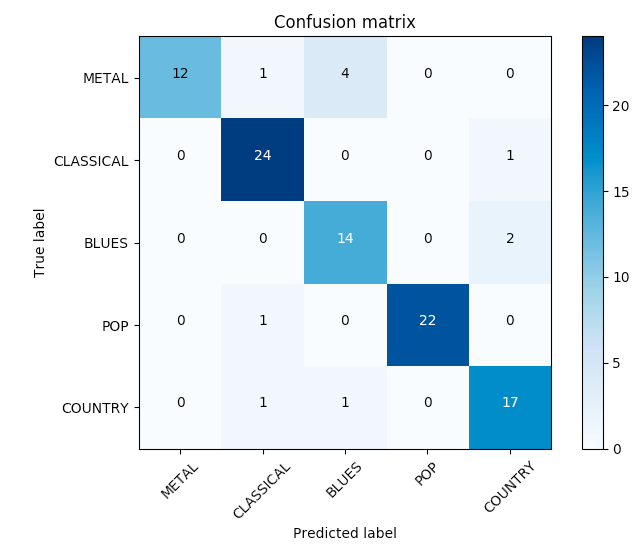
\includegraphics[scale=0.2]{./figures/confusion_cnn.png}
\end{center}
\caption
{
Confusion matrix for Convolutional Neural Network.
}
\label{fig:big_picture5}
\end{figure}

\begin{figure}
\begin{center}
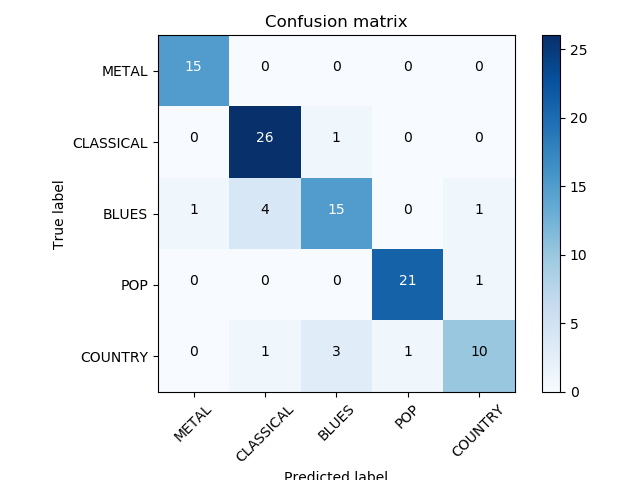
\includegraphics[scale=0.2]{./figures/confusion_sc.png}
\end{center}
\caption
{
Confusion matrix for Super Classifier.
}
\label{fig:big_picture5}
\end{figure}

\section{Conclusion}\label{sec:conclusion}
In conclusion, we implemented 7 different classifiers for music genre classification and it is fair to state that all the classifiers performed well, which is expected since we used 5 distinctive genres. It is observed that simple and easy to implement approaches such as k-NN and k-Means did worse than other more complicated classifiers such as SVMs or Neural Networks. Our goal was to achieve accuracy around 90\% and we were able to accomplish that goal with Convolutional Neural Networks. We also observed that it was easy to beat 80\% accuracy for 5 genres of music and the easiest genres to classify or distingush were classical and metal. Other than that, most of the classifiers had problems with classifying country or blues music.

